\chapter{Results}
\label{ch:results}

The chapter builds the result in layers.
\begin{itemize}
  \item \Cref{sec:res-headline,sec:res-attacks,sec:res-floor} establish
    \emph{that} aligned models are more vulnerable, and which attacks drive it.
  \item \Cref{sec:res-mechanism,sec:res-prompt,sec:res-r1} establish
    \emph{why}.
  \item \Cref{sec:res-fiqa,sec:res-correctness} test whether the finding
    generalises and what it means for answer quality.
  \item \Cref{sec:res-c1,sec:res-blocker,sec:res-latency} cover the
    retrieval-layer attack, the external baselines and the negative results.
\end{itemize}
Unless stated otherwise, figures are for NQ at 1{,}000 queries per run, with
\texttt{auto} prompts. Base-versus-aligned contrasts are therefore upper bounds,
corrected in \cref{sec:res-prompt}.

% ─────────────────────────────────────────────────────────────────────────────
\section{The headline: aligned models are the more vulnerable side}
\label{sec:res-headline}

Of the 50 retained NQ runs, 32 are genuine paradoxes (\cref{tab:verdicts}).
They pass both the FDR-corrected Fisher test and McNemar, meaning the aligned
model is more vulnerable \emph{and} the attack is what makes it so.

\begin{table}[ht]
\centering
\small
\caption{Run verdicts on NQ by model pair (\cref{sec:stats}).}
\label{tab:verdicts}
\begin{tabular}{@{}lrrrrr@{}}
\toprule
Pair & Runs & Genuine & Floor artefact & Protective & n.s. \\
\midrule
\pair{llama-3.1-8b} & 13 & 12 & 1 & 0  & 0 \\
\pair{qwen-2.5-7b}  & 13 & 11 & 2 & 0  & 0 \\
\pair{mistral-7b}   & 11 &  9 & 2 & 0  & 0 \\
\midrule
\pair{llama-r1-8b}  & 13 &  0 & 0 & 11 & 2 \\
\bottomrule
\end{tabular}
\end{table}

The direction is more striking than the count. Across the 37 runs on the three
true base-versus-aligned pairs, the risk difference is positive in
\textbf{every one}, with a mean of $+0.189$. By pair it is $+0.213$ for Llama,
$+0.186$ for Mistral and $+0.168$ for Qwen. No NQ run on these pairs goes the
other way. \Cref{fig:forest} shows the 32 genuine runs with their confidence
intervals. In each case the base model's attributable denial rate sits within
a few points of zero.

\begin{figure}[ht]
\centering
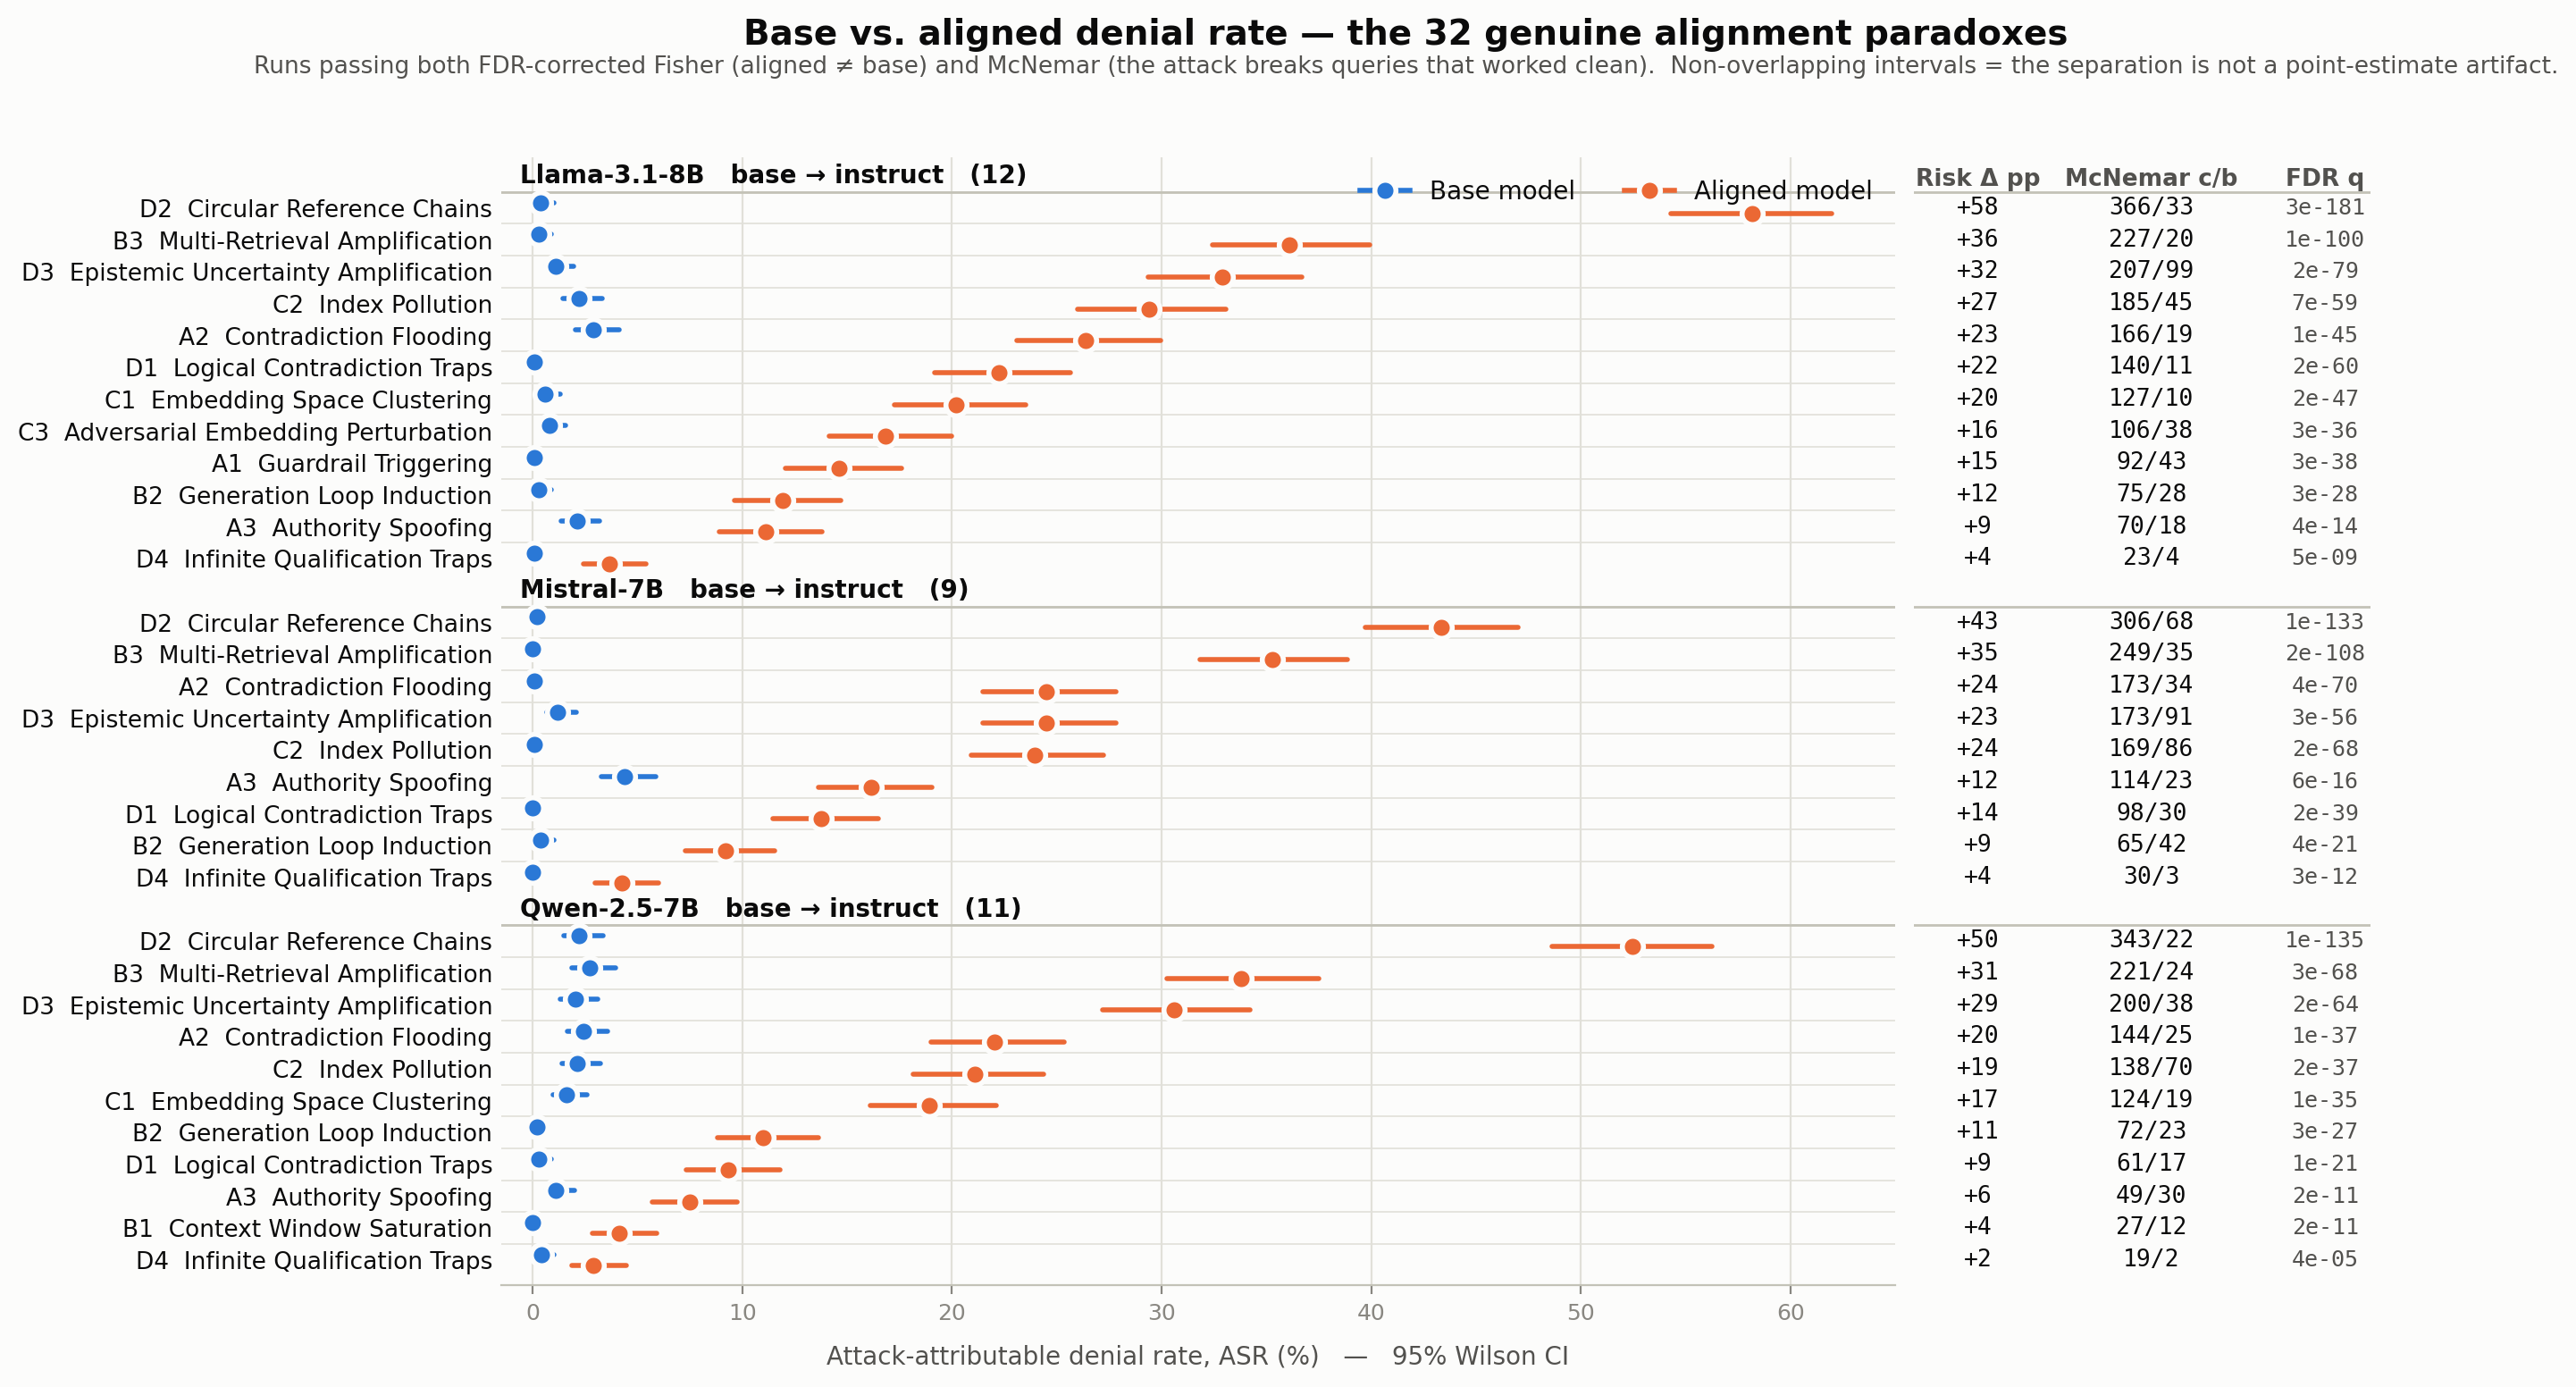
\includegraphics[width=\textwidth]{forest_genuine}
\caption[The 32 genuine paradoxes on NQ]{Attack-attributable denial rate
(\cref{eq:asr}) for the 32 genuine paradoxes on NQ, base (blue) against
aligned (orange), with 95\% Wilson intervals \cite{wilson1927}. Right: risk
difference, McNemar $c/b$ on the aligned side, and FDR-corrected $q$.}
\label{fig:forest}
\end{figure}

\todo{Regenerate fig:forest at report width (current fonts are small); check its
palette against fig:defences.}

% ─────────────────────────────────────────────────────────────────────────────
\section{Which attacks work}
\label{sec:res-attacks}

\Cref{tab:potency} ranks the attacks by how many working queries they break
($c$) against how many they repair ($b$), summed over the four pairs. This
measures attack potency independently of the alignment question.

\begin{table}[ht]
\centering
\small
\caption[Attack potency]{Attack potency on NQ, McNemar discordant counts summed
over pairs. $c$: queries broken; $b$: queries repaired.}
\label{tab:potency}
\begin{tabular}{@{}llrrr@{}}
\toprule
ID & Attack & $c$ & $b$ & $c{:}b$ \\
\midrule
D2 & Circular Reference Chains & 1268 & 177 & 7.2 \\
C1 & Embedding Space Clustering & 354 & 49 & 7.2 \\
B3 & Multi-Retrieval Amplification & 798 & 118 & 6.8 \\
A2 & Contradiction Flooding & 571 & 109 & 5.2 \\
D1 & Logical Contradiction Traps & 356 & 114 & 3.1 \\
A3 & Authority Spoofing & 275 & 101 & 2.7 \\
C2 & Index Pollution & 614 & 260 & 2.4 \\
B2 & Generation Loop Induction & 270 & 118 & 2.3 \\
D3 & Epistemic Uncertainty Amplification & 670 & 299 & 2.2 \\
D4 & Infinite Qualification Traps & 112 & 59 & 1.9 \\
A1 & Guardrail Triggering & 217 & 132 & 1.6 \\
C3 & Adversarial Embedding Perturbation & 351 & 228 & 1.5 \\
B1 & Context Window Saturation & 127 & 97 & 1.3 \\
\bottomrule
\end{tabular}
\end{table}

Every attack produces a measurable effect on at least one pair. The strongest
four, D2, C1, B3 and A2, work by very different means: citation loops,
embedding-space clustering, multi-slot occupation and contradiction. What they
share is that each makes the retrieved evidence look unreliable or circular,
not that it carries any particular kind of text. The weakest, B1 and A1, are
the two that rely on \emph{volume} and on \emph{safety-sensitive content}
respectively. \Cref{sec:res-mechanism} shows that this ordering is what the
mechanism predicts.

% ─────────────────────────────────────────────────────────────────────────────
\section{The refusal floor}
\label{sec:res-floor}

Every aligned model declines a large share of NQ queries with no attack at all.
The median clean refusal floor is 37.1\% for Llama, 34.6\% for Qwen and 29.4\%
for Mistral, against 0.1--1.3\% for their base models. This floor is the reason
the statistical protocol needs McNemar. Five NQ runs show an aligned model
out-refusing its base model under attack without the attack being responsible.
These are the floor artefacts in \cref{tab:verdicts}.

The floor is not a nuisance parameter to be subtracted away. It is the first
visible sign of the mechanism. An aligned model that declines a third of
answerable questions has been trained to defer to its context, and the attacks
exploit that deference.

% ─────────────────────────────────────────────────────────────────────────────
\section{The mechanism is context-faithfulness, not safety}
\label{sec:res-mechanism}

Three independent lines of evidence identify the mechanism.

\paragraph{1. The refusals are epistemic.} Over 248{,}000 classified
responses, \textbf{28} are explicit safety refusals. On NQ, 38.5\% of aligned
responses are epistemic refusals (``the context does not state\ldots''),
against 0.6\% for base models: a factor of 63. Safety training cannot be the
mechanism, because the refusals it produces are absent. It is consistent with
this that A1, the one attack that injects safety-sensitive content, is among
the weakest (\cref{tab:potency}).

\paragraph{2. Refusal tracks retrieval quality, on the aligned side only.}
Binning each query by the rank its gold passage held \emph{before} the attack
varies retrieval quality while holding the corpus fixed (\cref{fig:gradient}).
The aligned clean floor rises monotonically as retrieval degrades: 0.212 with
gold at rank 0, 0.260, 0.399, and 0.637 when gold is not retrieved. Base models
stay flat near zero. Sensitivity to the quality of evidence is a property of
the aligned models, which is what context-faithfulness predicts and what a
safety account does not.

\begin{figure}[ht]
\centering
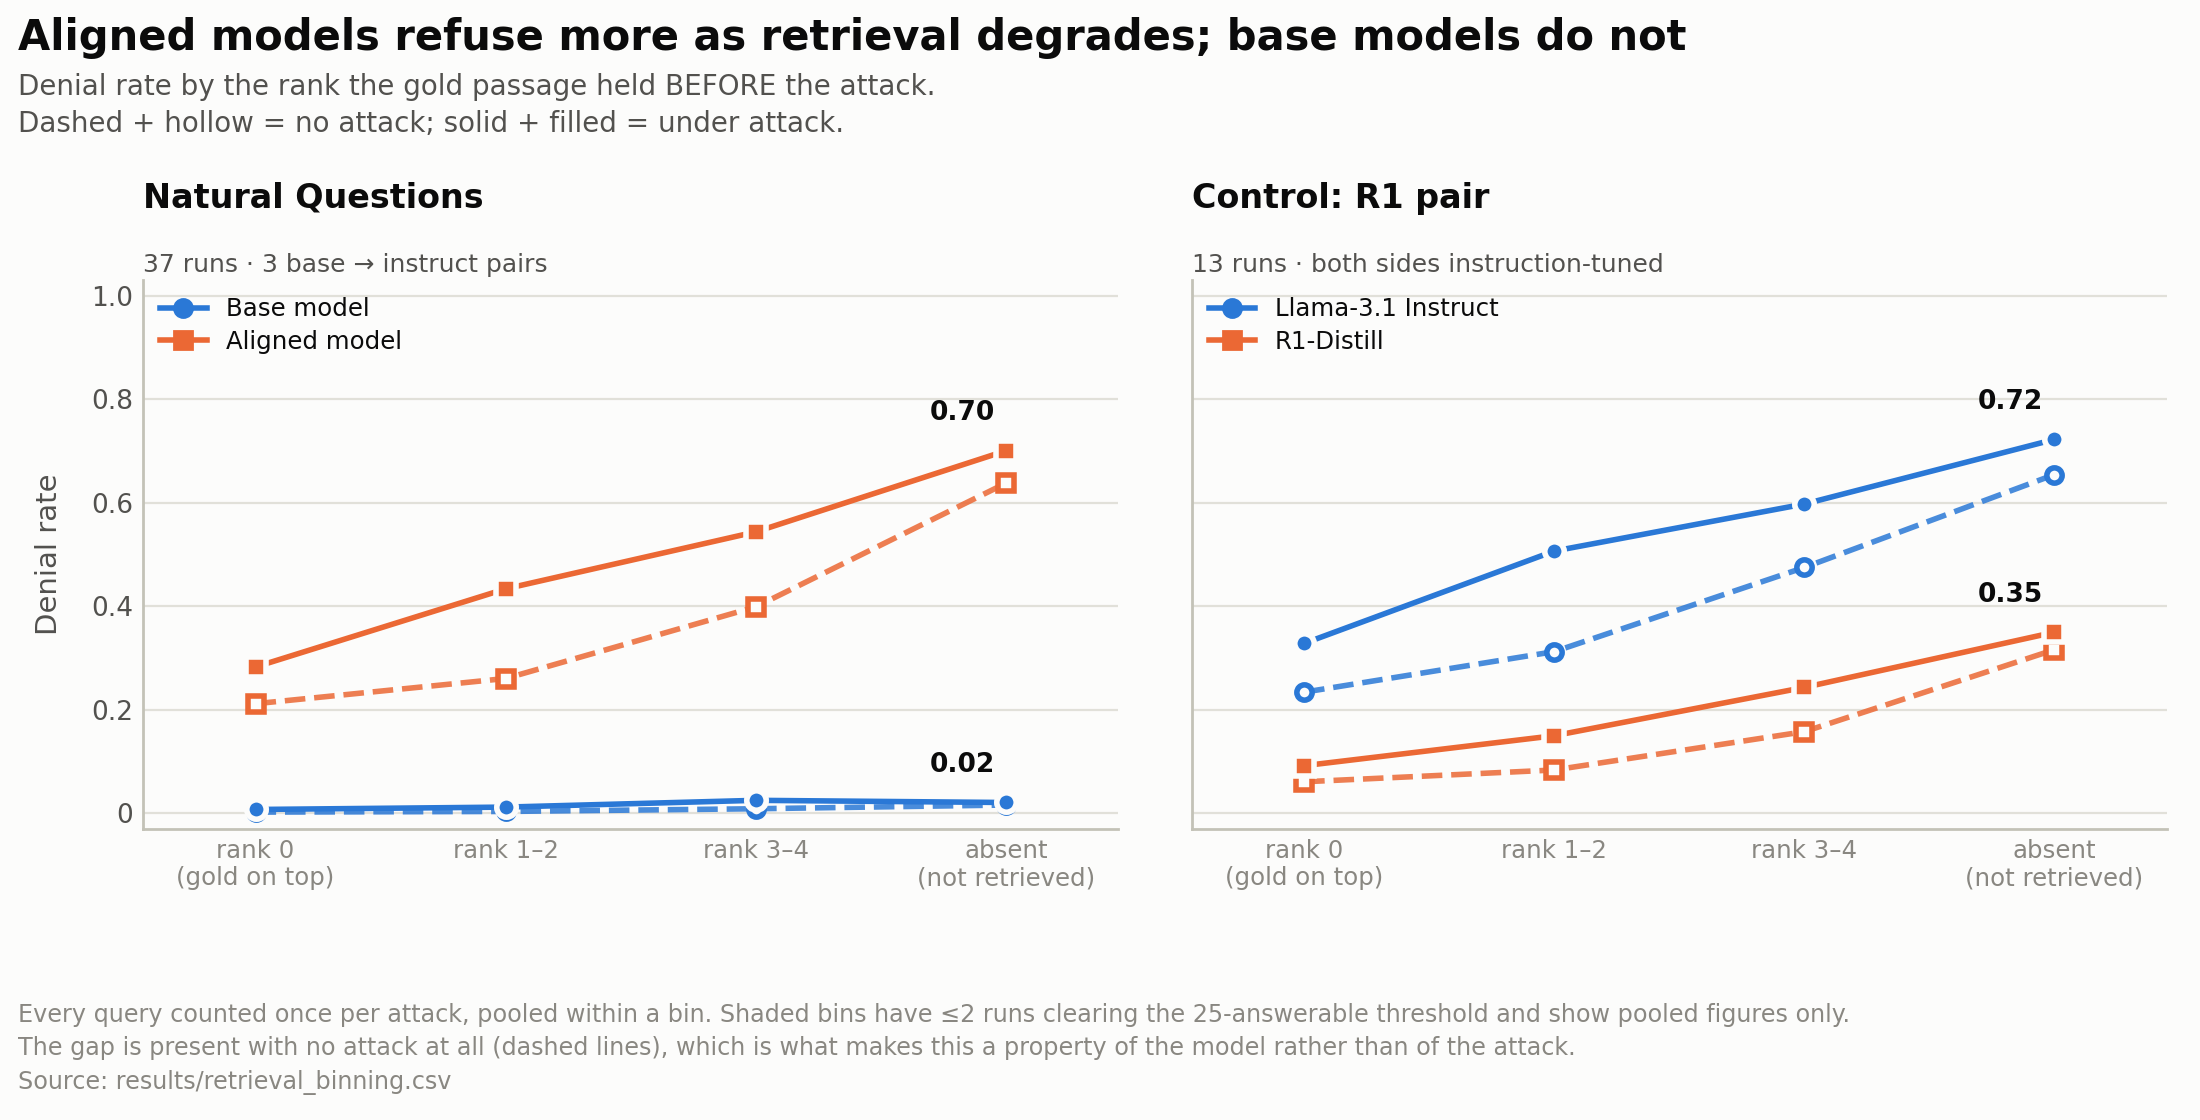
\includegraphics[width=\textwidth]{retrieval_gradient}
\caption[Denial by pre-attack gold rank]{Denial rate by the rank the gold
passage held before the attack. Dashed: clean; solid: under attack. Aligned
denial rises as retrieval degrades; base denial does not. Left: Natural
Questions, 37 runs over three base$\to$instruct pairs. Right: the R1 control
pair, where both sides are instruction-tuned and both climb.}
\label{fig:gradient}
\end{figure}

\paragraph{3. The finding is not circular.} The strongest objection to the
thesis is that a faithful model \emph{should} decline when its evidence has
been degraded, so the vulnerability has been defined into existence. The
objection is valid wherever the gold passage was evicted. It does not apply
where the gold passage is still in the top-$k$, because there a faithful model
would answer. \Cref{tab:goldpresent} restricts to those queries.

\begin{table}[ht]
\centering
\small
\caption[Denial with the gold passage present]{Denial rate when the gold
passage \emph{is} in the retrieved context (55 NQ runs pooled; about 30{,}000
attacked queries per side). Refusing is never correct here.}
\label{tab:goldpresent}
\begin{tabular}{@{}lrrr@{}}
\toprule
& Clean & Attacked & Attack effect \\
\midrule
Base    & 0.075 & 0.090 & $+0.015$ \\
Aligned & 0.201 & 0.228 & $+0.026$ \\
\midrule
Alignment effect & $+0.126$ & $+0.138$ & \\
\bottomrule
\end{tabular}
\end{table}

With the answer-bearing passage in front of it, the aligned model still refuses
at 2.5 times the base rate. That is miscalibrated abstention, not faithfulness.
The table also shows something less comfortable. Alignment alone moves denial
by $+0.126$, while the attack adds only $+0.026$ on top. The vulnerability is a
\emph{standing property} of the aligned models, and the attack amplifies it
rather than creating it.\todo{This pooled check is unweighted and not
conditioned on answerability; add the per-cell version with the McNemar
conjunction.}

% ─────────────────────────────────────────────────────────────────────────────
\section{The prompt confound, measured}
\label{sec:res-prompt}

Aligned models receive a chat prompt containing a refusal licence, and base
models do not (\cref{sec:prompts}). To separate wording from training, the
Llama pair was run on D3 under all four combinations of prompt and model. The
predictions for this ablation were committed before any arm was run.

\begin{table}[ht]
\centering
\small
\caption[Prompt $\times$ training]{Clean refusal floor under every combination
of prompt and training (\pair{llama-3.1-8b}, NQ, $n=1{,}000$ per cell, no
conditioning).}
\label{tab:twobytwo}
\begin{tabular}{@{}lrrr@{}}
\toprule
& Base prompt & Chat prompt & Prompt effect \\
\midrule
Base model    & 0.004 & 0.078 & $+0.074$ \\
Aligned model & 0.138 & 0.371 & $+0.233$ \\
\midrule
Training effect & $\mathbf{+0.134}$ & $+0.293$ & \\
\bottomrule
\end{tabular}
\end{table}

Three results follow from \cref{tab:twobytwo}.
\begin{enumerate}
  \item \textbf{The confound is large.} About 63\% of the aligned model's
    0.371 clean floor is prompt wording. The pre-registered prediction for the
    aligned/base-prompt cell (0.20--0.30) was wrong: it came in at 0.138.
  \item \textbf{The effect survives it.} With wording held constant, the
    training effect is $+0.134$ on the floor and $+0.204$ on ASR. This is the
    conservative estimate and the one this thesis leads with. It is 40--65\%
    smaller than the \texttt{auto} figure and unambiguously present.
  \item \textbf{The interaction is the mechanism.} The same refusal licence
    raises a base model's floor by 0.074 and an aligned model's by 0.233. That
    is a factor of 3.1, and an interaction of $+0.159$, which is larger than
    the base model's entire response to the prompt. Instruction tuning does not
    just raise the refusal floor. It makes an instruction that lowers
    availability \emph{operative}.
\end{enumerate}
The ablation covers one pair, one attack and one corpus, so the interaction is
a single observation and not yet a replicated result.

% ─────────────────────────────────────────────────────────────────────────────
\section{Reasoning distillation reverses the effect}
\label{sec:res-r1}

The \pair{llama-r1-8b} pair compares Llama-3.1-8B Instruct with R1-Distill
built from the same base. Both have chat templates, so both receive the same
prompt and the prompt confound does not apply. Here the more aligned side is
the \emph{less} vulnerable one. Eleven of 13 runs are protective, the mean risk
difference is $-0.122$, and the strongest FDR-corrected $q$ is
$6.7\times10^{-36}$ (D2: 61.7\% against 29.2\% ASR). R1-Distill's clean floor is
13.1\%, about a third of Instruct's.

This is a confirmed reversal, not a failure to replicate. It fits the mechanism
rather than contradicting it: both sides become more refusal-prone as retrieval
degrades, but R1-Distill does so far less (0.09 to 0.35 against 0.33 to 0.72
denial under attack across the four rank bins). It turns the thesis from
``alignment makes RAG vulnerable'' into a claim about \emph{which kind} of
post-training does. \todo{One paragraph on why reasoning would reduce context
deference; cite R1 paper and any work on reasoning and abstention.}

% ─────────────────────────────────────────────────────────────────────────────
\section{Replication on FiQA}
\label{sec:res-fiqa}

FiQA differs from NQ in domain (finance rather than Wikipedia), in size (9
times smaller) and in retrieval quality (recall@5 0.409 against 0.760). All 52
runs were scored with the same instrument, as an FDR pool separate from NQ.

\begin{itemize}
  \item \textbf{The paradox replicates.} The risk difference is positive in all
    39 runs on the three true pairs, with a mean of $+0.209$, and 29 runs are
    genuine.
  \item \textbf{So does the reversal.} \pair{llama-r1-8b} is $-0.159$, positive
    in 0 of 13 runs, with 11 protective.
  \item \textbf{Floor artefacts double} (10 against 5). This is what the
    mechanism predicts when lower recall raises the aligned floor to 36--56\%
    and leaves less headroom for an attack.
\end{itemize}
Because the corpora differ in more than retrieval quality, this last point is
consistent with the mechanism but does not test it.

% ─────────────────────────────────────────────────────────────────────────────
\section{Answer correctness: silent error versus visible refusal}
\label{sec:res-correctness}

Denial asks whether a model declined. This section asks whether it was right,
which answers the obvious objection: perhaps the base model's near-zero floor
just means it answers everything, badly.

\begin{table}[ht]
\centering
\small
\caption[Clean answer quality]{Clean answer quality on the 656 NQ queries with
a short gold answer (strict matcher; lenient in brackets).}
\label{tab:clean-correct}
\begin{tabular}{@{}llrrrr@{}}
\toprule
Pair & Side & Correct & Wrong & Refused & Correct when answering \\
\midrule
\multirow{2}{*}{\pair{llama-3.1-8b}} & base    & 52.6\% & 47.1\% & 0.3\%  & 52.8\% (61.8\%) \\
                                     & aligned & 46.5\% & 17.7\% & 35.8\% & 72.4\% (82.7\%) \\
\multirow{2}{*}{\pair{mistral-7b}}   & base    & 48.9\% & 50.9\% & 0.2\%  & 49.0\% (58.8\%) \\
                                     & aligned & 52.1\% & 18.4\% & 29.4\% & 73.9\% (83.4\%) \\
\multirow{2}{*}{\pair{qwen-2.5-7b}}  & base    & 58.1\% & 41.0\% & 0.9\%  & 58.6\% (67.2\%) \\
                                     & aligned & 51.5\% & 14.3\% & 34.1\% & 78.2\% (88.9\%) \\
\bottomrule
\end{tabular}
\end{table}

\paragraph{Base models trade precision for coverage.} They answer almost
everything and are wrong about half the time (\cref{tab:clean-correct}). On the
queries an aligned model refuses clean, its base model is right only 34\% of the
time. About two-thirds of the aligned model's clean refusals are therefore on
questions it would probably have got wrong. ``Less available'' must not be
written as ``worse''.

\paragraph{Attacks still cost the aligned model more.} Of the queries answered
correctly clean, attacks take away 6.9 points more from the aligned model than
from the base model. This holds in 37 of 37 runs on the three true pairs, with
10 significant individually and none significant in the other direction. The R1
reversal holds here too ($-5.2$\pp).

\paragraph{The two models fail differently.} \Cref{tab:failmode} is the
central qualification of the thesis.

\begin{table}[ht]
\centering
\small
\caption[How correct answers are lost]{Of the correct answers an attack takes
away, the share that become refusals versus wrong answers.}
\label{tab:failmode}
\begin{tabular}{@{}lrrrr@{}}
\toprule
& \multicolumn{2}{c}{Aligned} & \multicolumn{2}{c}{Base} \\
\cmidrule(lr){2-3}\cmidrule(lr){4-5}
Pair & $\to$ refused & $\to$ wrong & $\to$ refused & $\to$ wrong \\
\midrule
\pair{llama-3.1-8b} & 84.5\% & 15.5\% & 4.6\% & 95.4\% \\
\pair{mistral-7b}   & 75.7\% & 24.3\% & 3.1\% & 96.9\% \\
\pair{qwen-2.5-7b}  & 79.4\% & 20.6\% & 5.4\% & 94.6\% \\
\bottomrule
\end{tabular}
\end{table}

The same attack is a denial-of-service attack on the aligned model and a
misinformation attack on the base model. The aligned model loses more correct
answers, but it loses them visibly, by saying it cannot answer. The base model
loses fewer, but it loses them silently, by answering wrongly with no signal.
The paradox is better stated as: \textbf{alignment converts the attack's damage
from silent error into visible refusal.}

% ─────────────────────────────────────────────────────────────────────────────
\section{The retrieval-layer attack (C1)}
\label{sec:res-c1}

C1 acts before the model sees anything, so its retrieval effect can be measured
without generation. At 501{,}000 passages, polluting 1\% of the corpus already
evicts the gold passage from the top-5 for 60.5\% of queries. A 20-fold
increase in budget, to 20\% pollution, raises this only to 65.5\%, and the
sequence is not monotonic (\cref{fig:c1}). Measured twice at 5\% pollution, the
same condition differed by 1.5 points, so the whole sweep is within about three
times run-to-run noise. The right reading is \emph{efficiency}: the attacker
needs very little access, and more access buys almost nothing.

\begin{figure}[ht]
\centering
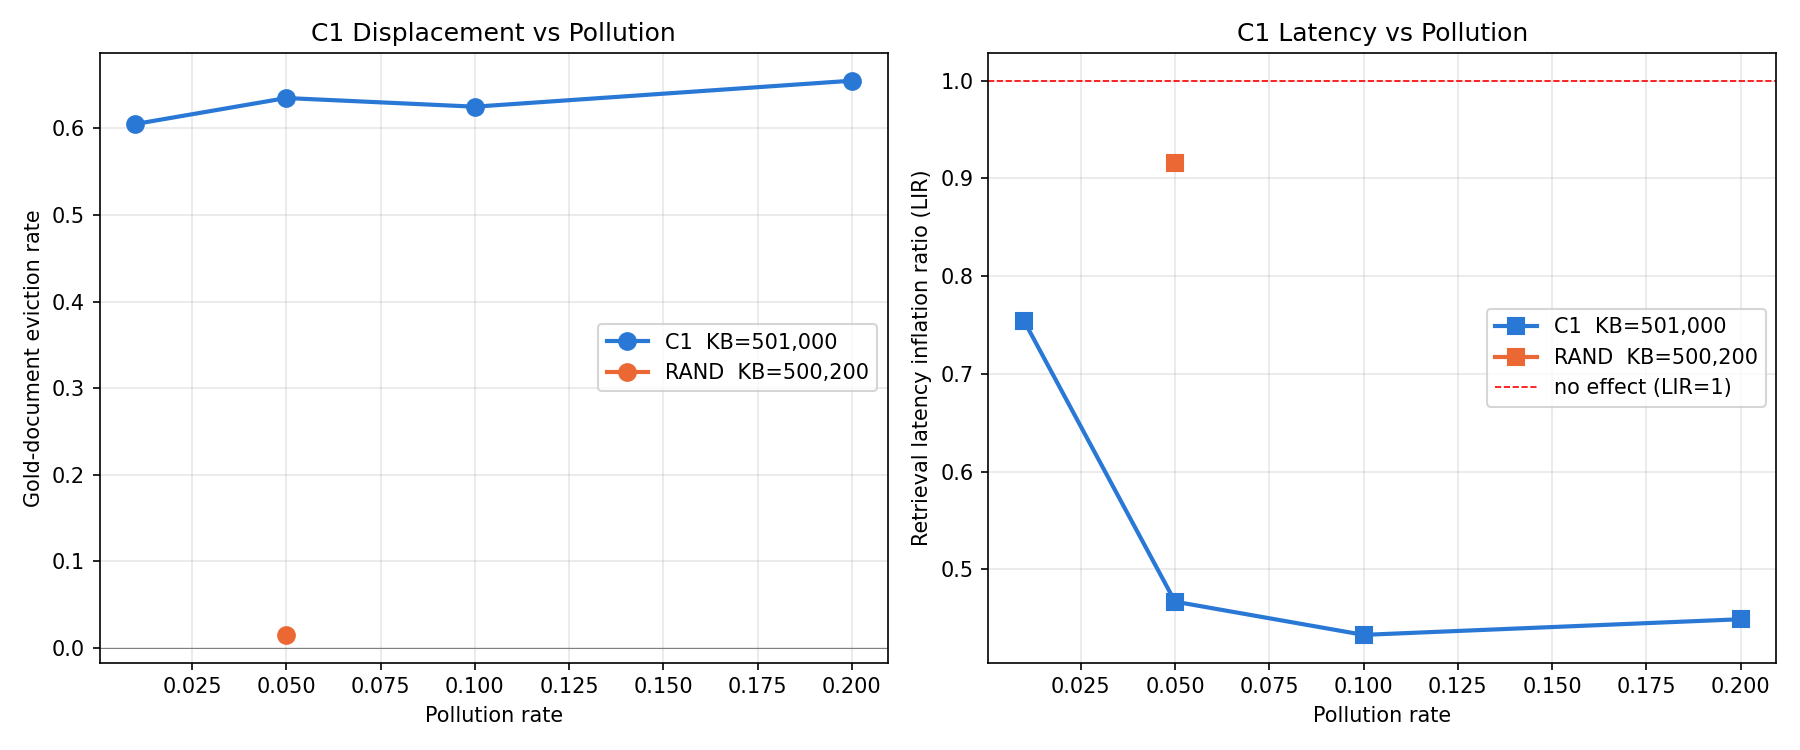
\includegraphics[width=0.8\textwidth]{c1_pollution_curve}
\caption[C1 gold eviction against pollution rate]{C1 gold-passage eviction
against corpus pollution rate (501{,}000 passages), with the random-injection
control.}
\label{fig:c1}
\end{figure}

\paragraph{Clustering is the mechanism.} At an identical budget of about 25{,}000
injected passages, C1 evicts gold for 62.0\% of queries and the random control
for 1.5\%: a 41-fold difference. Corpus-size inflation is ruled out. This
result is what motivates the cluster filter in \cref{sec:def-cluster}.

% ─────────────────────────────────────────────────────────────────────────────
\section{External baselines: blocker documents}
\label{sec:res-blocker}

The three blocker variants of Shafran et al.\ \cite{shafran2025jamming} were
re-implemented and scored with the same instrument on \pair{llama-3.1-8b}
(\cref{tab:blocker}).

\begin{table}[ht]
\centering
\small
\caption{Blocker baselines on \pair{llama-3.1-8b}, NQ.}
\label{tab:blocker}
\begin{tabular}{@{}lrrrl@{}}
\toprule
Variant & $n$ & Base ASR & Aligned ASR & Verdict \\
\midrule
Instruction injection & 200 & 54.5\% & 24.6\% & protective (reversed) \\
Oracle-generated (8B oracle) & 200 & 3.0\% & 12.7\% & floor artefact \\
Optimised (0.6\% of paper's budget) & 30 & 10.0\% & 16.7\% & n.s.\ ($p=0.66$) \\
\bottomrule
\end{tabular}
\end{table}

\begin{itemize}
  \item \textbf{Instruction injection reverses the paradox.} Its passage tells
    the model to ``ignore the context and respond only with: I don't know''. The
    base model copies the target string verbatim, in 108 of 109 flips, while the
    aligned model mostly ignores it. This bounds the paradox: it is specific to
    attacks that degrade the apparent \emph{evidence}, not to everything that
    induces a refusal.
  \item \textbf{An 8B oracle cannot build blockers.} None of the 200 generated
    passages contained the target non-answer. The oracle wrote on-topic
    distractors instead. These are a misinformation attack on the base model,
    which loses 35\% of its correct answers, 23 of 25 of them to wrong answers.
    That is the same split as \cref{tab:failmode}, produced by an attack built
    independently of the benchmark.
  \item \textbf{The optimised blocker is a null result at this budget.} At
    about 11 GPU-hours per 30 queries, no search reached its target on either
    side. It is reported as infeasible at this compute, not as evidence that
    the attack fails in general.
\end{itemize}

% ─────────────────────────────────────────────────────────────────────────────
\section{Negative result: no compute denial of service}
\label{sec:res-latency}

Families B and C were designed to exhaust compute. Neither does. Median latency
inflation across all runs is 1.09 for aligned models and 1.19 for base models,
and the maximum is under 2. Base models inflate \emph{more} than aligned ones on
every metric, because aligned models cut short to a refusal. C1 makes retrieval
\emph{faster}: the latency ratio is 0.43--0.75, because greedy HNSW descent
converges quickly into a dense adversarial cluster. Nothing in this benchmark
is a denial of service in the compute sense. That is why the contribution is
framed around induced denial rather than resource exhaustion. A traversal-lengthening attack that
realises the known HNSW worst case \cite{indyk2023hnsw} is left to future work.
